% Options for packages loaded elsewhere
\PassOptionsToPackage{unicode}{hyperref}
\PassOptionsToPackage{hyphens}{url}
%
\documentclass[
]{article}
\usepackage{amsmath,amssymb}
\usepackage{iftex}
\ifPDFTeX
  \usepackage[T1]{fontenc}
  \usepackage[utf8]{inputenc}
  \usepackage{textcomp} % provide euro and other symbols
\else % if luatex or xetex
  \usepackage{unicode-math} % this also loads fontspec
  \defaultfontfeatures{Scale=MatchLowercase}
  \defaultfontfeatures[\rmfamily]{Ligatures=TeX,Scale=1}
\fi
\usepackage{lmodern}
\ifPDFTeX\else
  % xetex/luatex font selection
\fi
% Use upquote if available, for straight quotes in verbatim environments
\IfFileExists{upquote.sty}{\usepackage{upquote}}{}
\IfFileExists{microtype.sty}{% use microtype if available
  \usepackage[]{microtype}
  \UseMicrotypeSet[protrusion]{basicmath} % disable protrusion for tt fonts
}{}
\makeatletter
\@ifundefined{KOMAClassName}{% if non-KOMA class
  \IfFileExists{parskip.sty}{%
    \usepackage{parskip}
  }{% else
    \setlength{\parindent}{0pt}
    \setlength{\parskip}{6pt plus 2pt minus 1pt}}
}{% if KOMA class
  \KOMAoptions{parskip=half}}
\makeatother
\usepackage{xcolor}
\usepackage[margin=1in]{geometry}
\usepackage{color}
\usepackage{fancyvrb}
\newcommand{\VerbBar}{|}
\newcommand{\VERB}{\Verb[commandchars=\\\{\}]}
\DefineVerbatimEnvironment{Highlighting}{Verbatim}{commandchars=\\\{\}}
% Add ',fontsize=\small' for more characters per line
\usepackage{framed}
\definecolor{shadecolor}{RGB}{248,248,248}
\newenvironment{Shaded}{\begin{snugshade}}{\end{snugshade}}
\newcommand{\AlertTok}[1]{\textcolor[rgb]{0.94,0.16,0.16}{#1}}
\newcommand{\AnnotationTok}[1]{\textcolor[rgb]{0.56,0.35,0.01}{\textbf{\textit{#1}}}}
\newcommand{\AttributeTok}[1]{\textcolor[rgb]{0.13,0.29,0.53}{#1}}
\newcommand{\BaseNTok}[1]{\textcolor[rgb]{0.00,0.00,0.81}{#1}}
\newcommand{\BuiltInTok}[1]{#1}
\newcommand{\CharTok}[1]{\textcolor[rgb]{0.31,0.60,0.02}{#1}}
\newcommand{\CommentTok}[1]{\textcolor[rgb]{0.56,0.35,0.01}{\textit{#1}}}
\newcommand{\CommentVarTok}[1]{\textcolor[rgb]{0.56,0.35,0.01}{\textbf{\textit{#1}}}}
\newcommand{\ConstantTok}[1]{\textcolor[rgb]{0.56,0.35,0.01}{#1}}
\newcommand{\ControlFlowTok}[1]{\textcolor[rgb]{0.13,0.29,0.53}{\textbf{#1}}}
\newcommand{\DataTypeTok}[1]{\textcolor[rgb]{0.13,0.29,0.53}{#1}}
\newcommand{\DecValTok}[1]{\textcolor[rgb]{0.00,0.00,0.81}{#1}}
\newcommand{\DocumentationTok}[1]{\textcolor[rgb]{0.56,0.35,0.01}{\textbf{\textit{#1}}}}
\newcommand{\ErrorTok}[1]{\textcolor[rgb]{0.64,0.00,0.00}{\textbf{#1}}}
\newcommand{\ExtensionTok}[1]{#1}
\newcommand{\FloatTok}[1]{\textcolor[rgb]{0.00,0.00,0.81}{#1}}
\newcommand{\FunctionTok}[1]{\textcolor[rgb]{0.13,0.29,0.53}{\textbf{#1}}}
\newcommand{\ImportTok}[1]{#1}
\newcommand{\InformationTok}[1]{\textcolor[rgb]{0.56,0.35,0.01}{\textbf{\textit{#1}}}}
\newcommand{\KeywordTok}[1]{\textcolor[rgb]{0.13,0.29,0.53}{\textbf{#1}}}
\newcommand{\NormalTok}[1]{#1}
\newcommand{\OperatorTok}[1]{\textcolor[rgb]{0.81,0.36,0.00}{\textbf{#1}}}
\newcommand{\OtherTok}[1]{\textcolor[rgb]{0.56,0.35,0.01}{#1}}
\newcommand{\PreprocessorTok}[1]{\textcolor[rgb]{0.56,0.35,0.01}{\textit{#1}}}
\newcommand{\RegionMarkerTok}[1]{#1}
\newcommand{\SpecialCharTok}[1]{\textcolor[rgb]{0.81,0.36,0.00}{\textbf{#1}}}
\newcommand{\SpecialStringTok}[1]{\textcolor[rgb]{0.31,0.60,0.02}{#1}}
\newcommand{\StringTok}[1]{\textcolor[rgb]{0.31,0.60,0.02}{#1}}
\newcommand{\VariableTok}[1]{\textcolor[rgb]{0.00,0.00,0.00}{#1}}
\newcommand{\VerbatimStringTok}[1]{\textcolor[rgb]{0.31,0.60,0.02}{#1}}
\newcommand{\WarningTok}[1]{\textcolor[rgb]{0.56,0.35,0.01}{\textbf{\textit{#1}}}}
\usepackage{graphicx}
\makeatletter
\def\maxwidth{\ifdim\Gin@nat@width>\linewidth\linewidth\else\Gin@nat@width\fi}
\def\maxheight{\ifdim\Gin@nat@height>\textheight\textheight\else\Gin@nat@height\fi}
\makeatother
% Scale images if necessary, so that they will not overflow the page
% margins by default, and it is still possible to overwrite the defaults
% using explicit options in \includegraphics[width, height, ...]{}
\setkeys{Gin}{width=\maxwidth,height=\maxheight,keepaspectratio}
% Set default figure placement to htbp
\makeatletter
\def\fps@figure{htbp}
\makeatother
\setlength{\emergencystretch}{3em} % prevent overfull lines
\providecommand{\tightlist}{%
  \setlength{\itemsep}{0pt}\setlength{\parskip}{0pt}}
\setcounter{secnumdepth}{-\maxdimen} % remove section numbering
\ifLuaTeX
  \usepackage{selnolig}  % disable illegal ligatures
\fi
\IfFileExists{bookmark.sty}{\usepackage{bookmark}}{\usepackage{hyperref}}
\IfFileExists{xurl.sty}{\usepackage{xurl}}{} % add URL line breaks if available
\urlstyle{same}
\hypersetup{
  pdftitle={Práctica dirigida 2},
  hidelinks,
  pdfcreator={LaTeX via pandoc}}

\title{Práctica dirigida 2}
\author{}
\date{\vspace{-2.5em}}

\begin{document}
\maketitle

{
\setcounter{tocdepth}{4}
\tableofcontents
}

\includegraphics[width=0.3\linewidth]{logoPUCP}

\textbf{FACULTAD DE CIENCIAS SOCIALES - PUCP}

\hypertarget{curso-pol-278---estaduxedstica-para-el-anuxe1lisis-poluxedtico-1-semestre-2024---2}{%
\subsection{\texorpdfstring{Curso: POL 278 - Estadística para el
análisis político 1 \textbar{} Semestre 2024 - 2
}{Curso: POL 278 - Estadística para el análisis político 1 \textbar{} Semestre 2024 - 2  }}\label{curso-pol-278---estaduxedstica-para-el-anuxe1lisis-poluxedtico-1-semestre-2024---2}}

\begin{center}\rule{0.5\linewidth}{0.5pt}\end{center}

\hypertarget{quuxe9-es-el-anuxe1lisis-descriptivo}{%
\section{\texorpdfstring{\textbf{1.¿Qué es el análisis
descriptivo?}}{1.¿Qué es el análisis descriptivo?}}\label{quuxe9-es-el-anuxe1lisis-descriptivo}}

\begin{center}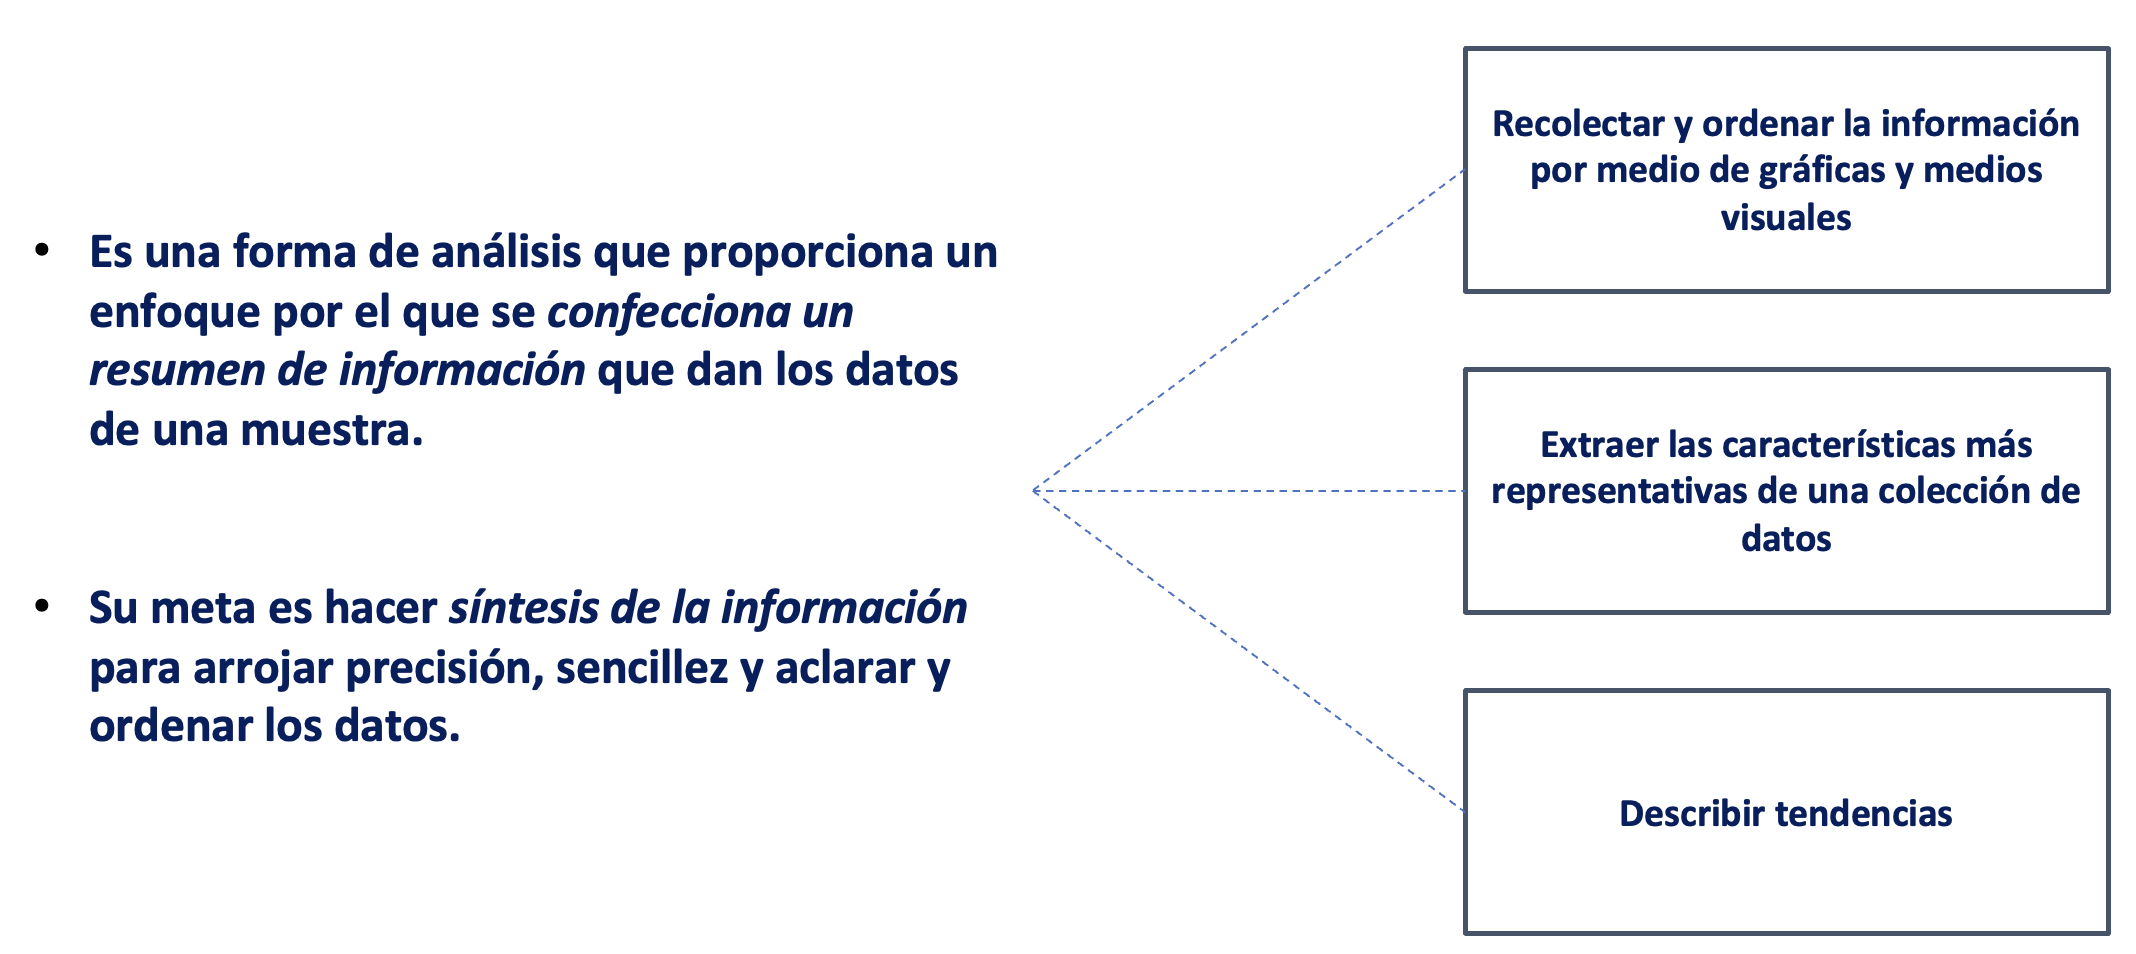
\includegraphics[width=0.8\linewidth]{pd2_QSAnalisisDesc} \end{center}

\hypertarget{nivel-de-medida-de-una-variable}{%
\section{\texorpdfstring{\textbf{2.Nivel de medida de una
variable}}{2.Nivel de medida de una variable}}\label{nivel-de-medida-de-una-variable}}

\begin{center}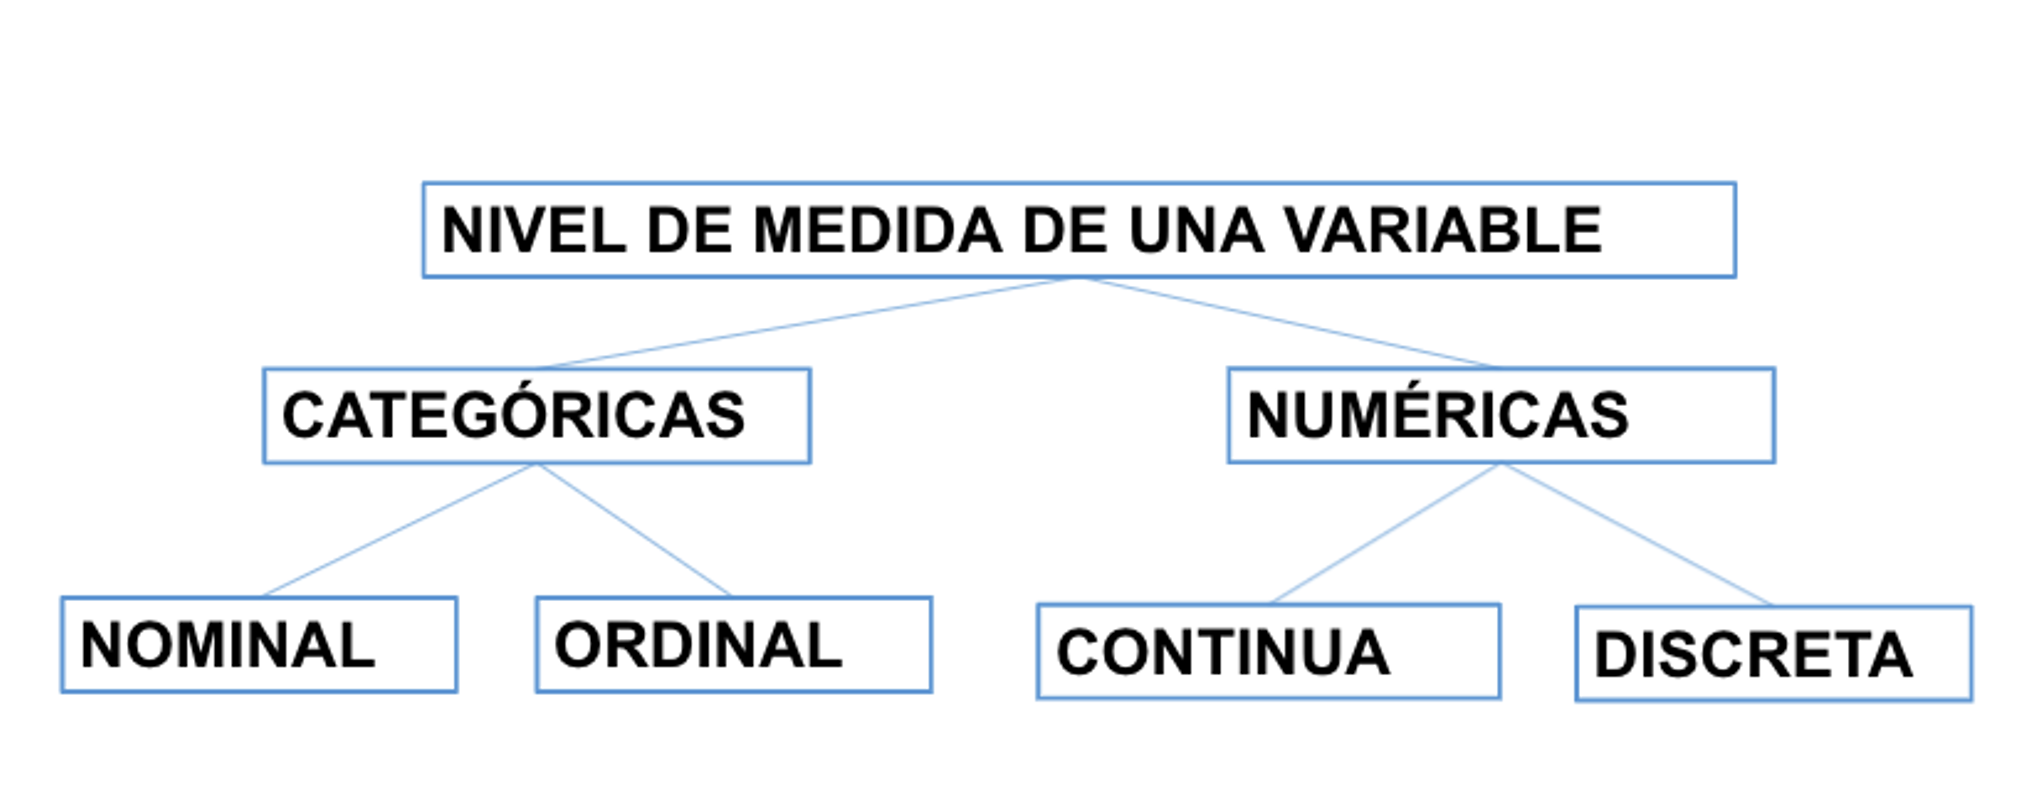
\includegraphics[width=0.5\linewidth]{pd2_medVar} \end{center}

\hypertarget{importancia-de-visualizaciuxf3n-de-datos}{%
\section{\texorpdfstring{\textbf{3.Importancia de visualización de
datos}}{3.Importancia de visualización de datos}}\label{importancia-de-visualizaciuxf3n-de-datos}}

Debido al crecimiento de la big data en los últimos años surgieron
nuevas necesidades para comprender los análisis masivos de datos de una
forma simple y escalable. Es entonces cuando se dirige la atención a
desarrollar nuevas técnicas gráficas en distintas plataformas (ejemplos
a continuación), tanto softwares como librerías de código
abierto\footnote{\url{https://www.data-to-viz.com/caveat/pie.html}}, tal
es el caso de ggplot2 en R.

\begin{center}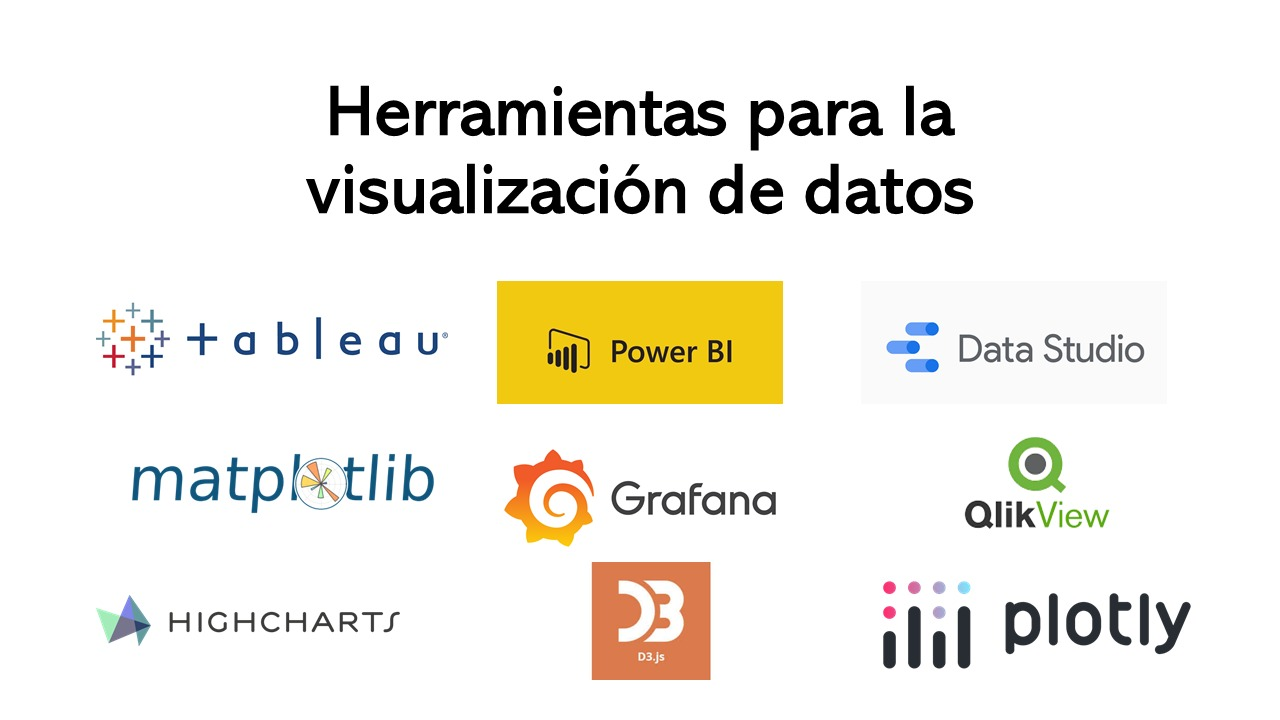
\includegraphics[width=0.9\linewidth]{pd2_herramientas} \end{center}

Este interés por desarrollar técnicas de análisis masivo de datos y la
comunicación de resultados cada vez más amigables y apta para todos los
públicos dio pie a nuevas especialidades dentro de la ciencia de datos,
como por ejemplo el data story telling

\begin{center}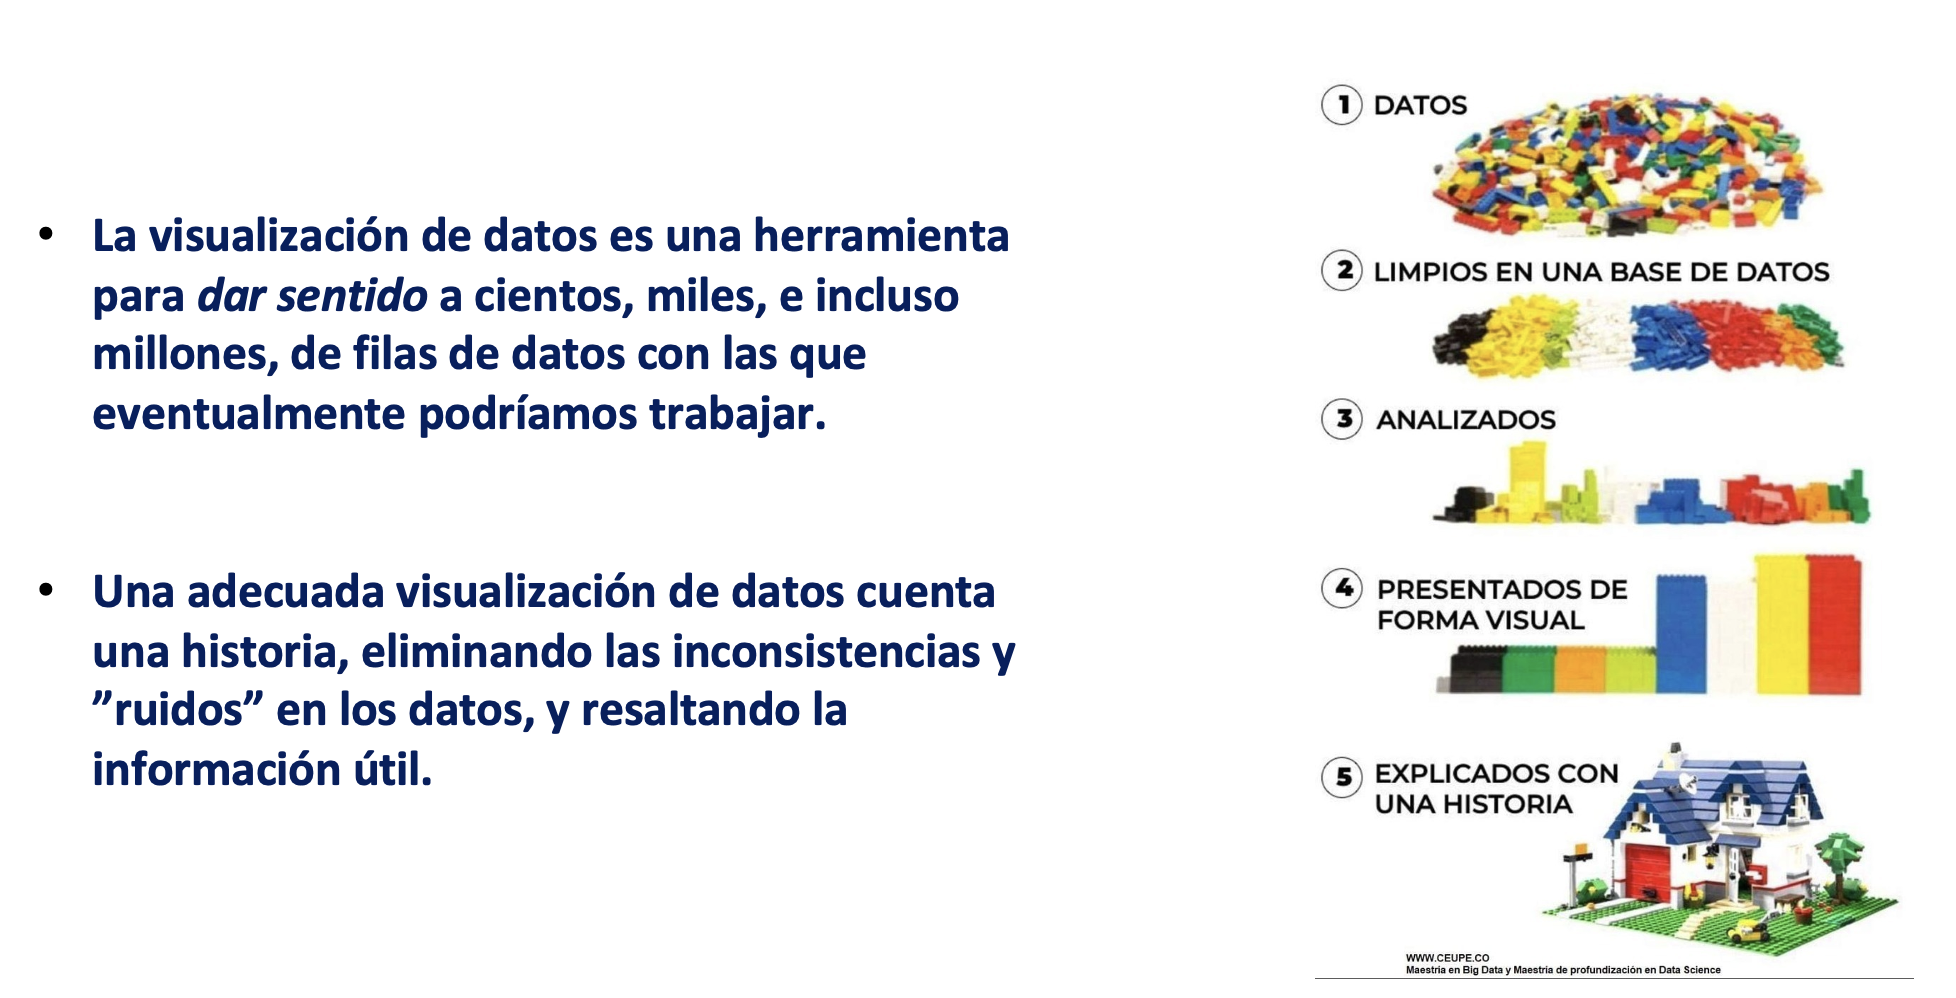
\includegraphics[width=0.9\linewidth]{pd2_datavis} \end{center}

\hypertarget{gruxe1ficos-por-tipo-de-variables}{%
\subsubsection{\texorpdfstring{\textbf{Gráficos por tipo de
variables:}}{Gráficos por tipo de variables:}}\label{gruxe1ficos-por-tipo-de-variables}}

\begin{center}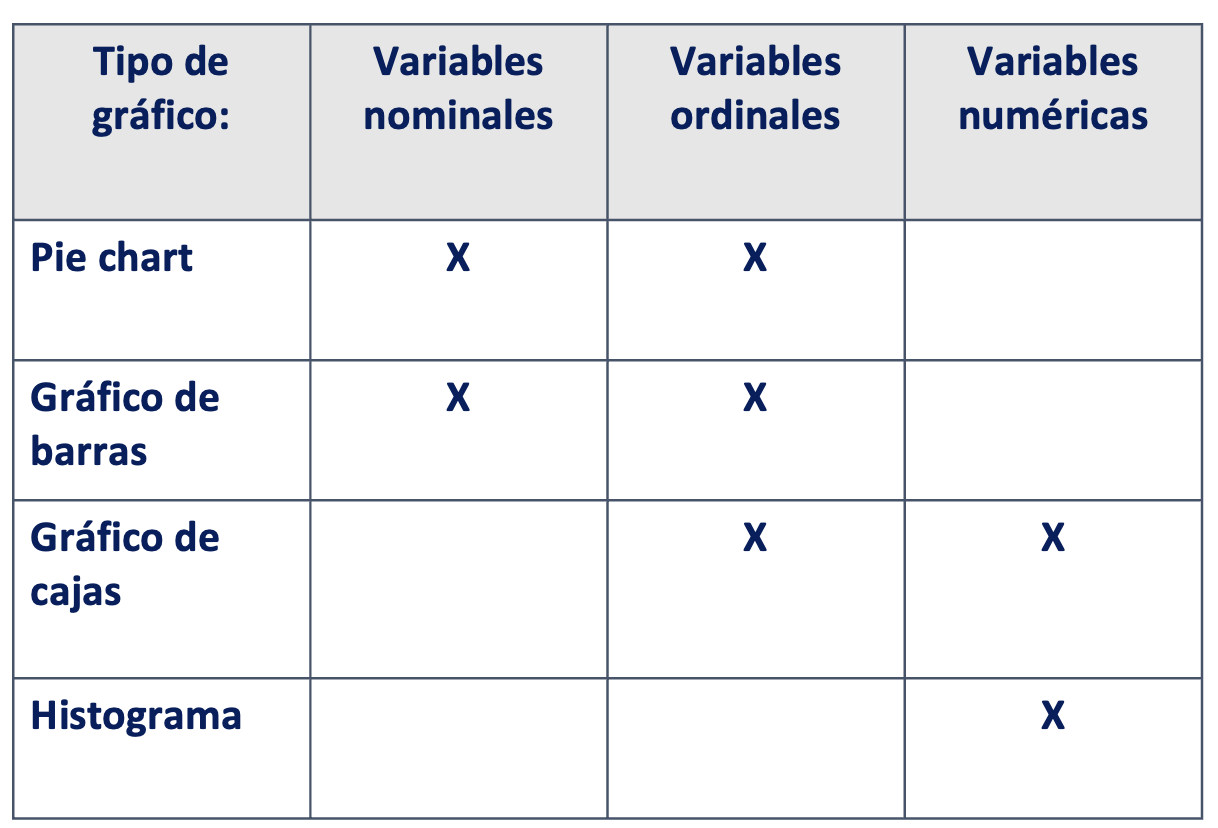
\includegraphics[width=0.6\linewidth]{pd2_GrafTipoVar} \end{center}

\hypertarget{anuxe1lisis-descriptivo}{%
\section{\texorpdfstring{\textbf{4.Análisis
descriptivo}}{4.Análisis descriptivo}}\label{anuxe1lisis-descriptivo}}

¿Cuál es la percepción de desigualdad en el Perú el 2024? 🤔

Para dar respuesta a la pregunta de investigación que guiara la práctica
dirigida analizaremos algunas de las variables que forman parte de la
Encuesta Nacional de Percepción de Desigualdades - ENADES 2024, que fue
elaborada por Instituto de Estudios Peruanos (IEP) y Oxfam. La encuesta
busca ahondar en la percepción de las diferentes formas de desigualdad
en el Perú e incorpora indicadores que permiten medir la magnitud de
brechas sociales y políticas como género, clase, entre otros.

Se eligieron algunas variables de la base de datos original y se dejaron
por fuera valores perdidos además de realizar otras modificaciones. Para
realizar alguna investigación se debe usar la base de datos original que
se encuentra en el siguiente
\href{https://peru.oxfam.org/ENADES-2024}{link}.

\begin{center}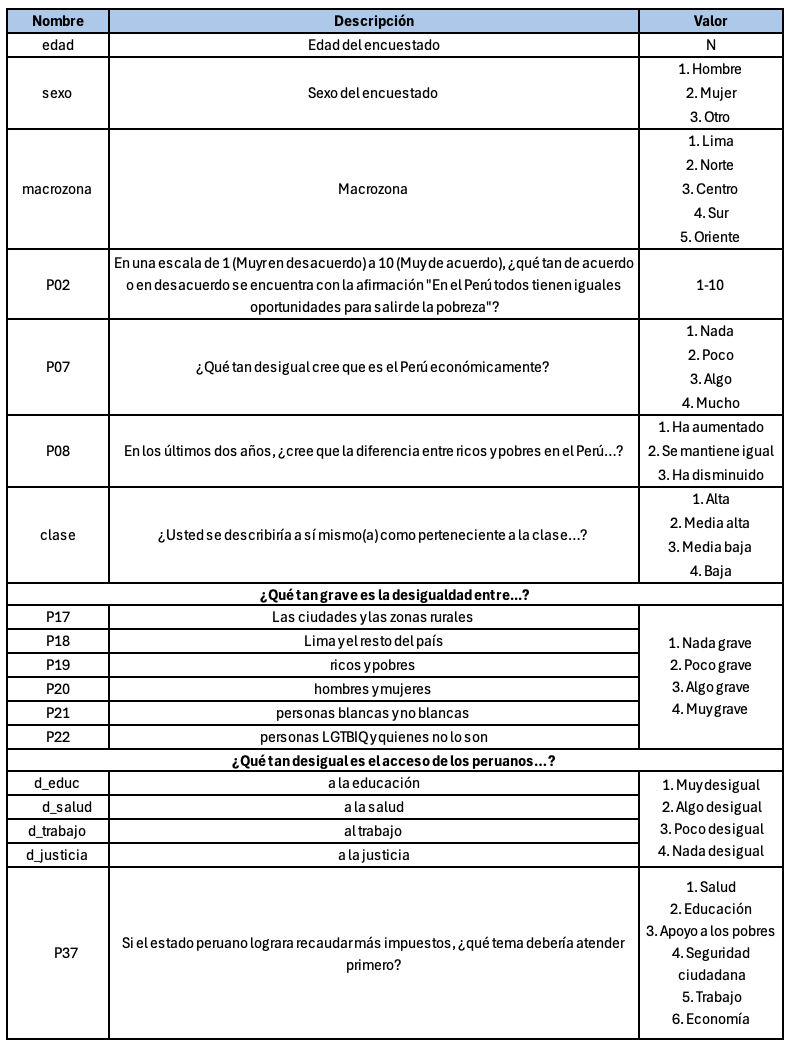
\includegraphics[width=1\linewidth]{diccionario_enades2024} \end{center}

\begin{Shaded}
\begin{Highlighting}[]
\FunctionTok{library}\NormalTok{(rio) }\CommentTok{\#Convocamos el paquete   }
\NormalTok{data}\OtherTok{=}\FunctionTok{import}\NormalTok{(}\StringTok{"pd2\_enades2024.xlsx"}\NormalTok{)}
\end{Highlighting}
\end{Shaded}

\begin{Shaded}
\begin{Highlighting}[]
\FunctionTok{str}\NormalTok{(data) }\CommentTok{\#revisamos las variables}
\end{Highlighting}
\end{Shaded}

\begin{verbatim}
## 'data.frame':    562 obs. of  18 variables:
##  $ edad      : num  19 40 47 20 37 27 36 37 35 19 ...
##  $ sexo      : num  1 2 2 2 2 2 2 1 1 1 ...
##  $ macrozona : num  4 3 4 4 4 4 3 4 4 4 ...
##  $ P02       : num  7 7 10 10 6 4 8 1 1 3 ...
##  $ P07       : num  4 1 4 4 4 2 4 4 4 3 ...
##  $ P08       : num  1 3 1 1 1 1 2 3 1 1 ...
##  $ clase     : num  3 3 3 3 3 4 3 3 4 3 ...
##  $ P17       : num  4 2 4 3 1 3 2 1 3 3 ...
##  $ P18       : num  3 2 3 4 2 3 3 1 3 3 ...
##  $ P19       : num  4 4 4 4 4 4 3 4 3 4 ...
##  $ P20       : num  3 1 3 3 3 3 3 1 2 3 ...
##  $ P21       : num  3 2 3 3 1 1 2 1 2 3 ...
##  $ P22       : num  2 3 3 3 3 1 3 1 2 3 ...
##  $ d_educ    : num  2 3 2 1 2 1 3 1 3 2 ...
##  $ d_salud   : num  1 1 1 2 2 1 2 1 1 1 ...
##  $ d_trabajo : num  2 3 1 1 1 3 3 1 1 2 ...
##  $ d_justicia: num  2 1 2 1 2 1 2 1 1 2 ...
##  $ P37       : num  2 1 2 6 3 2 4 1 2 2 ...
\end{verbatim}

\hypertarget{cuxf3mo-se-distribuye-la-percepciuxf3n-de-desigualdad-econuxf3mica-en-el-peruxfa}{%
\subsection{4.1 ¿Cómo se distribuye (\%)la percepción de desigualdad
económica en el
Perú?}\label{cuxf3mo-se-distribuye-la-percepciuxf3n-de-desigualdad-econuxf3mica-en-el-peruxfa}}

Usaremos la variable \textbf{P07}:

\texttt{¿Qué\ tan\ desigual\ cree\ que\ es\ el\ Perú\ económicamente?}

De acuerdo al diccionario de datos encontramos cuatro posibles
respuestas

\begin{itemize}
\tightlist
\item
  1:Nada
\item
  2:Poco
\item
  3:Algo
\item
  4:Mucho
\end{itemize}

\hypertarget{anuxe1lisis-de-una-variable-ordinal}{%
\subsubsection{\texorpdfstring{\textbf{Análisis de una variable
ordinal}}{Análisis de una variable ordinal}}\label{anuxe1lisis-de-una-variable-ordinal}}

Pasos para analizar una variable ordinal A. Identificar el tipo de
variable (str, class) B. Convertimos la variable al tipo de dato que
necesitamos dependiendo el caso C. Elaboramos un objeto que nos permita
ver preliminarmente los datos de la variable. D. Elaboramos un gráfico
que vaya acorde a la variable ordinal (gráfico de barras)

\begin{Shaded}
\begin{Highlighting}[]
\FunctionTok{library}\NormalTok{(dplyr) }\CommentTok{\#Convocamos el paquete}
\end{Highlighting}
\end{Shaded}

Comprobamos el tipo de dato que analizaremos

\begin{Shaded}
\begin{Highlighting}[]
\FunctionTok{class}\NormalTok{(data}\SpecialCharTok{$}\NormalTok{P07)}
\end{Highlighting}
\end{Shaded}

\begin{verbatim}
## [1] "numeric"
\end{verbatim}

Del diccionario de datos, sabemos que esta variable es \textbf{ordinal},
revisemos si los niveles tienen coherencia con las respuestas recogidas
en la encuesta.

\begin{Shaded}
\begin{Highlighting}[]
\NormalTok{data }\SpecialCharTok{\%\textgreater{}\%}
 \FunctionTok{group\_by}\NormalTok{(P07) }\SpecialCharTok{\%\textgreater{}\%}
 \FunctionTok{summarise}\NormalTok{(}\AttributeTok{Freq=}\FunctionTok{n}\NormalTok{()) }\CommentTok{\#Veamos los niveles de la variable}
\end{Highlighting}
\end{Shaded}

\begin{verbatim}
## # A tibble: 4 x 2
##     P07  Freq
##   <dbl> <int>
## 1     1    32
## 2     2   125
## 3     3    97
## 4     4   308
\end{verbatim}

💥 Etiquetamos y categorizamos como factor. Para ello usaremos el
comando \textbf{mutate}. Este comando forma parte del paquete dplyr. Lo
usaremos cada vez que se quiera modificar de alguna forma la data o
alguna variable en específico.

\begin{Shaded}
\begin{Highlighting}[]
\NormalTok{data }\OtherTok{=}\NormalTok{ data }\SpecialCharTok{\%\textgreater{}\%}
 \FunctionTok{mutate}\NormalTok{(}\AttributeTok{P07 =} \FunctionTok{factor}\NormalTok{(P07, }\AttributeTok{levels =} \DecValTok{1}\SpecialCharTok{:}\DecValTok{4}\NormalTok{, }\AttributeTok{labels =} \FunctionTok{c}\NormalTok{(}\StringTok{"Nada"}\NormalTok{, }\StringTok{"Poco"}\NormalTok{, }\StringTok{"Algo"}\NormalTok{, }\StringTok{"Mucho"}\NormalTok{), }\AttributeTok{ordered =} \ConstantTok{TRUE}\NormalTok{))}
\end{Highlighting}
\end{Shaded}

En este caso queremos que dentro de la variable P07 se almacene el
resultado de convertir P07 a factor y según los cuatro niveles que tiene
otorgar una etiqueta. Es así que lo que aparece como 1 será Nada, lo que
aparece como 2 será Poco, 3 será Algo y 4, Mucho.

Revisemos que el cambio se haya realizado correctamente usando el
comando \textbf{summarise} del paquete \texttt{dplyr}. Los resultados de
la tabla deben mantenerse, lo que varía debe ser la etiqueta de la
categoría.

\begin{Shaded}
\begin{Highlighting}[]
\NormalTok{data }\SpecialCharTok{\%\textgreater{}\%}
 \FunctionTok{group\_by}\NormalTok{(P07) }\SpecialCharTok{\%\textgreater{}\%}
 \FunctionTok{summarise}\NormalTok{(}\AttributeTok{Freq=}\FunctionTok{n}\NormalTok{())}
\end{Highlighting}
\end{Shaded}

\begin{verbatim}
## # A tibble: 4 x 2
##   P07    Freq
##   <ord> <int>
## 1 Nada     32
## 2 Poco    125
## 3 Algo     97
## 4 Mucho   308
\end{verbatim}

A primera vista, la tabla nos indica que la mayoría de los encuestados
(453) opina que hay mucha desigualdad económica en el país. Pero,
¿cuánto sería dicho resultado en porcentaje?

Podemos realizar una tabla de frecuencias y porcentajes agregando una
linea al comando anterior. Asimismo, para poder graficar los resultados
de las tablas, tendremos que almacenarlas en un objeto. Trabajemos con
esta tabla resumen y asignemosle el nombre \emph{\texttt{para\_grafico}}
para posteriormente llamarla al graficar.

Para agregar el porcentaje usaremos \textbf{mutate}. Recordemos que el
porcentaje sería el resultado de la frecuencia de la categoría sobre el
total. Debemos solicitarle a R que realice ese cálculo en cada fila.

\begin{Shaded}
\begin{Highlighting}[]
\NormalTok{para\_grafico}\OtherTok{=}\NormalTok{data }\SpecialCharTok{\%\textgreater{}\%}
 \FunctionTok{group\_by}\NormalTok{(P07) }\SpecialCharTok{\%\textgreater{}\%}
 \FunctionTok{summarize}\NormalTok{(}\AttributeTok{Freq=}\FunctionTok{n}\NormalTok{()) }\SpecialCharTok{\%\textgreater{}\%}
 \FunctionTok{mutate}\NormalTok{(}\AttributeTok{Porcentaje =}\NormalTok{ (Freq }\SpecialCharTok{/} \FunctionTok{sum}\NormalTok{(Freq))}\SpecialCharTok{*}\DecValTok{100}\NormalTok{)}
\end{Highlighting}
\end{Shaded}

Hemos creado un nuevo objeto llamado para\_grafico. Para poder
visualizarlo podemos llamarlo por su nombre. Siempre que almacenemos un
objeto, debemos llamarlo para poder visualizarlo.

\begin{Shaded}
\begin{Highlighting}[]
\NormalTok{para\_grafico}
\end{Highlighting}
\end{Shaded}

\begin{verbatim}
## # A tibble: 4 x 3
##   P07    Freq Porcentaje
##   <ord> <int>      <dbl>
## 1 Nada     32       5.69
## 2 Poco    125      22.2 
## 3 Algo     97      17.3 
## 4 Mucho   308      54.8
\end{verbatim}

Afirmamos que más del 50\% de los encuestados percibe que el país es muy
desigual económicamente.

También podemos analizar cómo cambia esto si solo seleccionamos los
casos de los encuestados/as menores de 30 años. Para ello haremos uso
del comando \textbf{filter}. Este comando necesita dos argumentos: a. La
variable sobre la cual se filtrará y b. la condición. En este caso la
variable es edad y la condición es ``menos a 30'' o \textless30.

\begin{Shaded}
\begin{Highlighting}[]
\NormalTok{data }\SpecialCharTok{\%\textgreater{}\%}
  \FunctionTok{filter}\NormalTok{(edad}\SpecialCharTok{\textless{}}\DecValTok{30}\NormalTok{)}\SpecialCharTok{\%\textgreater{}\%}
  \FunctionTok{group\_by}\NormalTok{(P07) }\SpecialCharTok{\%\textgreater{}\%}
  \FunctionTok{summarize}\NormalTok{(}\AttributeTok{Freq=}\FunctionTok{n}\NormalTok{()) }\SpecialCharTok{\%\textgreater{}\%}
  \FunctionTok{mutate}\NormalTok{(}\AttributeTok{Porcentaje =}\NormalTok{ (Freq }\SpecialCharTok{/} \FunctionTok{sum}\NormalTok{(Freq))}\SpecialCharTok{*}\DecValTok{100}\NormalTok{)}
\end{Highlighting}
\end{Shaded}

\begin{verbatim}
## # A tibble: 4 x 3
##   P07    Freq Porcentaje
##   <ord> <int>      <dbl>
## 1 Nada      7       4.35
## 2 Poco     30      18.6 
## 3 Algo     36      22.4 
## 4 Mucho    88      54.7
\end{verbatim}

Grafiquemos los resultados con \emph{\texttt{ggplot2}}

Nuestra variable es categórica, por lo tanto realizaremos el gráfico
acorde:

\begin{Shaded}
\begin{Highlighting}[]
\FunctionTok{library}\NormalTok{(ggplot2)}
\end{Highlighting}
\end{Shaded}

\begin{verbatim}
## Warning: package 'ggplot2' was built under R version 4.2.3
\end{verbatim}

\begin{Shaded}
\begin{Highlighting}[]
\FunctionTok{ggplot}\NormalTok{(para\_grafico, }\FunctionTok{aes}\NormalTok{(}\AttributeTok{x=}\NormalTok{P07, }\AttributeTok{y=}\NormalTok{Porcentaje, }\AttributeTok{fill=}\NormalTok{P07)) }\SpecialCharTok{+} 
\FunctionTok{geom\_bar}\NormalTok{(}\AttributeTok{stat =} \StringTok{"identity"}\NormalTok{) }\SpecialCharTok{+}
  \FunctionTok{theme\_bw}\NormalTok{()}
\end{Highlighting}
\end{Shaded}

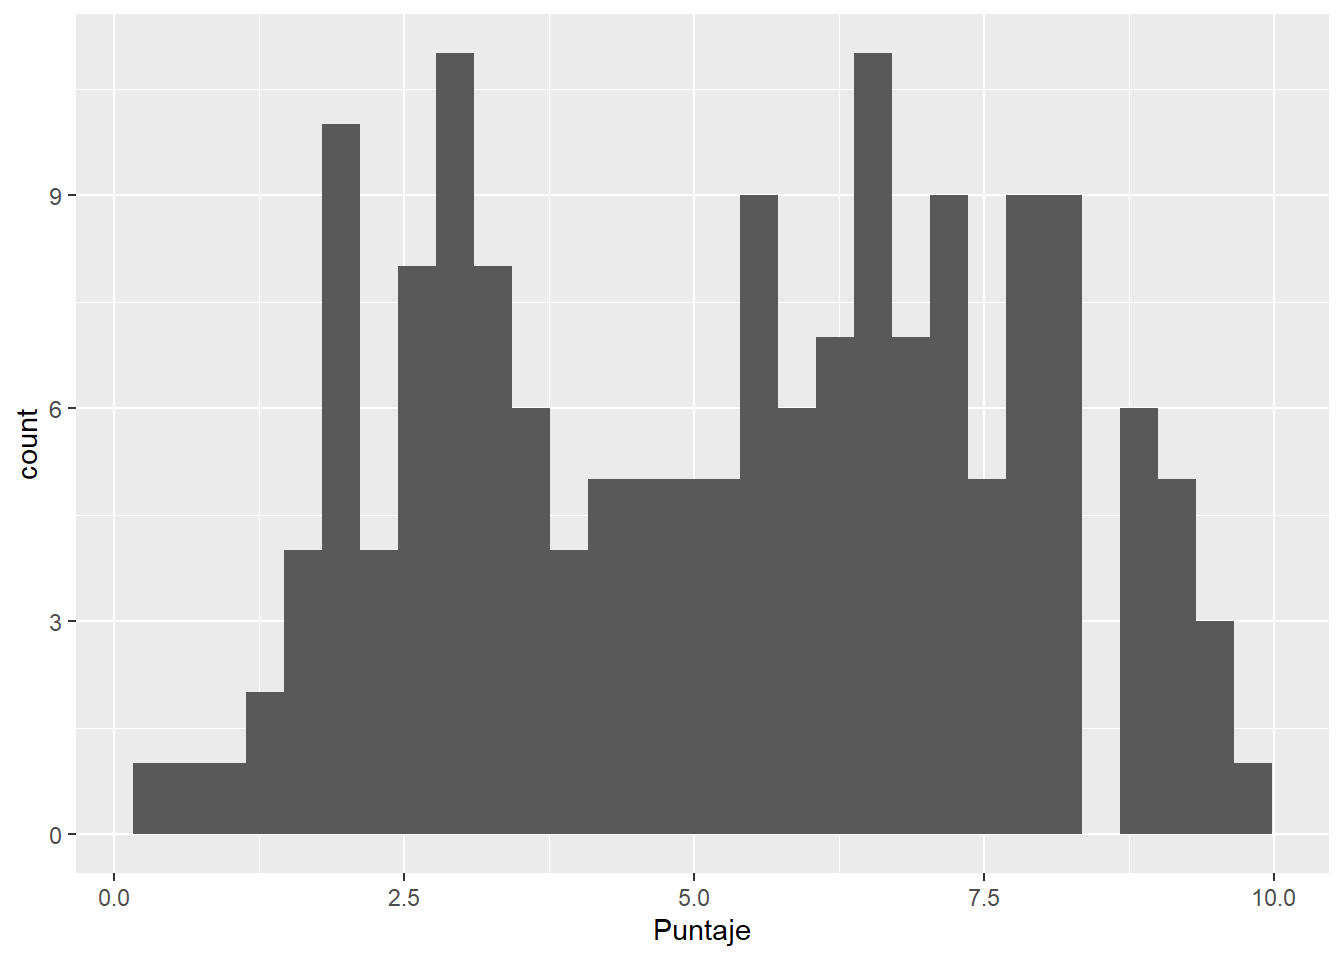
\includegraphics{pd2_files/figure-latex/unnamed-chunk-18-1.pdf}

Este es un gráfico básico, pero podemos personalizarlo\footnote{\url{https://cran.r-project.org/web/packages/tayloRswift/readme/README.html}}
según nuestros gustos.

\begin{Shaded}
\begin{Highlighting}[]
\FunctionTok{library}\NormalTok{(tayloRswift) }\CommentTok{\#opcional (una ventaja de que R sea software libre)}

\FunctionTok{ggplot}\NormalTok{(para\_grafico, }\FunctionTok{aes}\NormalTok{(}\AttributeTok{x=}\NormalTok{P07, }\AttributeTok{y=}\NormalTok{Porcentaje, }\AttributeTok{fill=}\NormalTok{P07)) }\SpecialCharTok{+} 
  \FunctionTok{geom\_bar}\NormalTok{(}\AttributeTok{stat =} \StringTok{"identity"}\NormalTok{)  }\SpecialCharTok{+}
  \FunctionTok{ggtitle}\NormalTok{(}\StringTok{"Percepción de desigualdad económica"}\NormalTok{) }\SpecialCharTok{+}
  \FunctionTok{xlab}\NormalTok{(}\StringTok{"¿Qué tan desigual cree que es el Perú económicamente"}\NormalTok{) }\SpecialCharTok{+} \FunctionTok{ylab}\NormalTok{(}\StringTok{"Porcentaje"}\NormalTok{)}\SpecialCharTok{+}
  \FunctionTok{geom\_text}\NormalTok{(}\FunctionTok{aes}\NormalTok{(}\AttributeTok{label=}\FunctionTok{round}\NormalTok{(Porcentaje,}\DecValTok{1}\NormalTok{)), }\AttributeTok{vjust=}\FloatTok{1.30}\NormalTok{, }\AttributeTok{color=}\StringTok{"black"}\NormalTok{, }\AttributeTok{size=}\DecValTok{3}\NormalTok{)}\SpecialCharTok{+}
  \FunctionTok{theme}\NormalTok{(}\AttributeTok{panel.background=}\FunctionTok{element\_rect}\NormalTok{(}\AttributeTok{fill =} \StringTok{"white"}\NormalTok{, }\AttributeTok{colour =} \StringTok{"white"}\NormalTok{)) }\SpecialCharTok{+}
  \FunctionTok{scale\_fill\_taylor}\NormalTok{(}\AttributeTok{palette =} \StringTok{"lover"}\NormalTok{) }\CommentTok{\#fearless, speakNow, Red}
\end{Highlighting}
\end{Shaded}

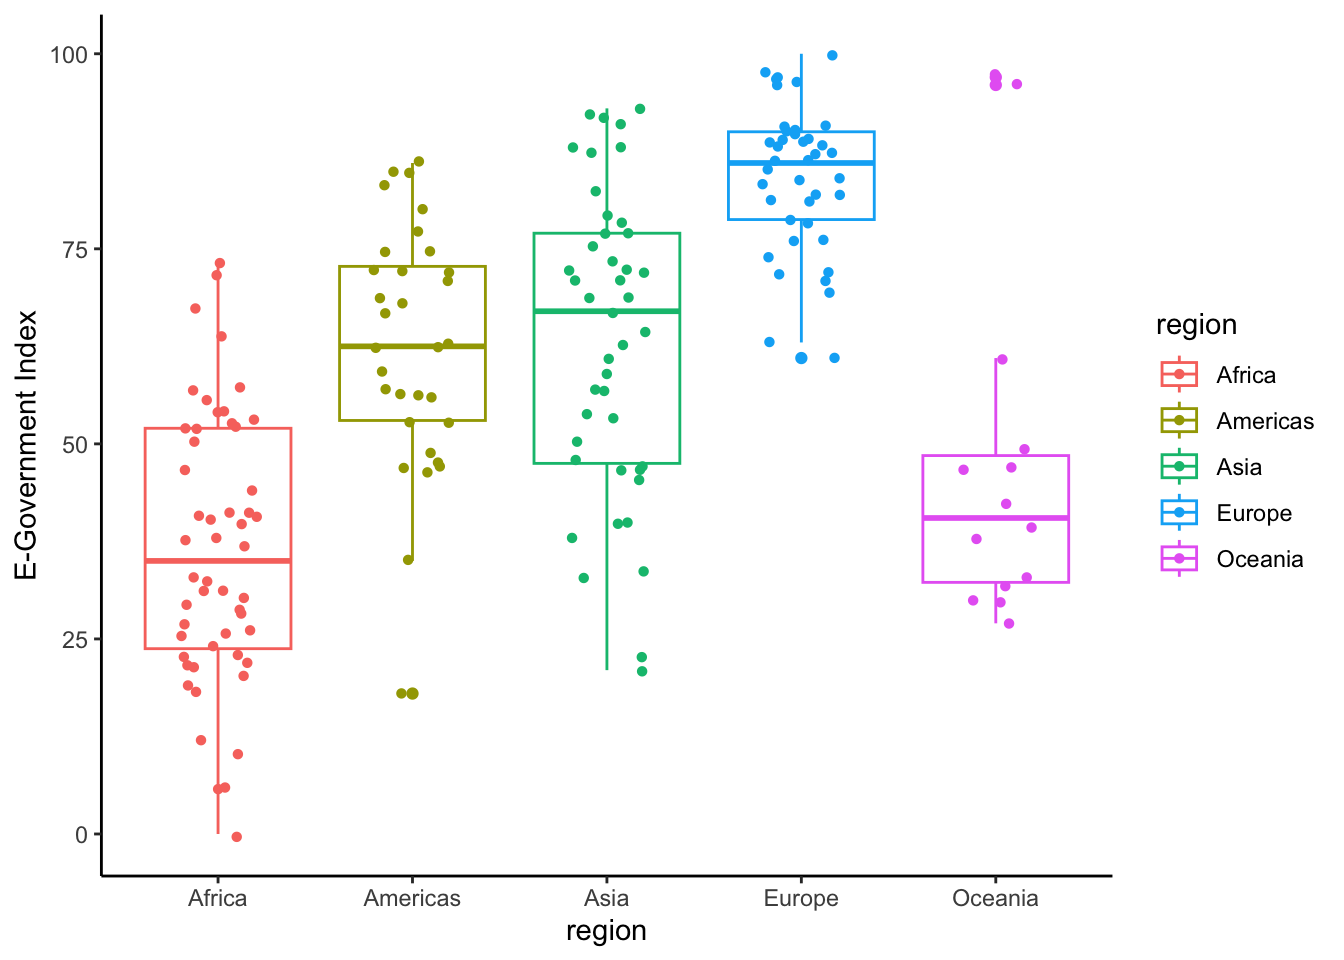
\includegraphics{pd2_files/figure-latex/unnamed-chunk-19-1.pdf}

El ejercicio de análisis descriptivo con variables numéricas lo
realizaremos con un indicador aditivo que crearemos a continuación.

\hypertarget{cuuxe1l-es-la-percepciuxf3n-de-la-desigualdad-en-calidad-de-vida-en-el-peruxfa}{%
\subsection{4.2 ¿Cuál es la percepción de la desigualdad en calidad de
vida en el
Perú?}\label{cuuxe1l-es-la-percepciuxf3n-de-la-desigualdad-en-calidad-de-vida-en-el-peruxfa}}

\hypertarget{indicador-proxy}{%
\subsubsection{\texorpdfstring{\textbf{Indicador
Proxy}}{Indicador Proxy}}\label{indicador-proxy}}

También llamado indicador indirecto, se usa ante la imposibilidad de
medir lo que efectivamente es de importancia. El indicador mide una
variable distinta a la que nos interesa de manera específica, pero
presenta una relación lo más directa posible con el fenómeno en estudio.

Un indicador proxy es una medición o señal indirecto que aproxima o
representa un fenómeno en la ausencia de una medición o señal directo.

\hypertarget{indicador-aditivo}{%
\subsubsection{\texorpdfstring{\textbf{Indicador
Aditivo}}{Indicador Aditivo}}\label{indicador-aditivo}}

Es una variable latente que se genera a través de la suma de un conjunto
de variables manifiestas u observables. Luego de la suma se procede a
aplicar una formula que genera que el valor máximo de la variable sea 1
y el mínimo sea 0. A partir de eso se puede multiplicar por cualquier
número para que el máximo cambie. Es así que si se multiplica por 10, el
indicador irá de 0 a 10; si se desea que el indicador sea de 0 a 50, se
debe multiplicar por 50; etc.

\begin{center}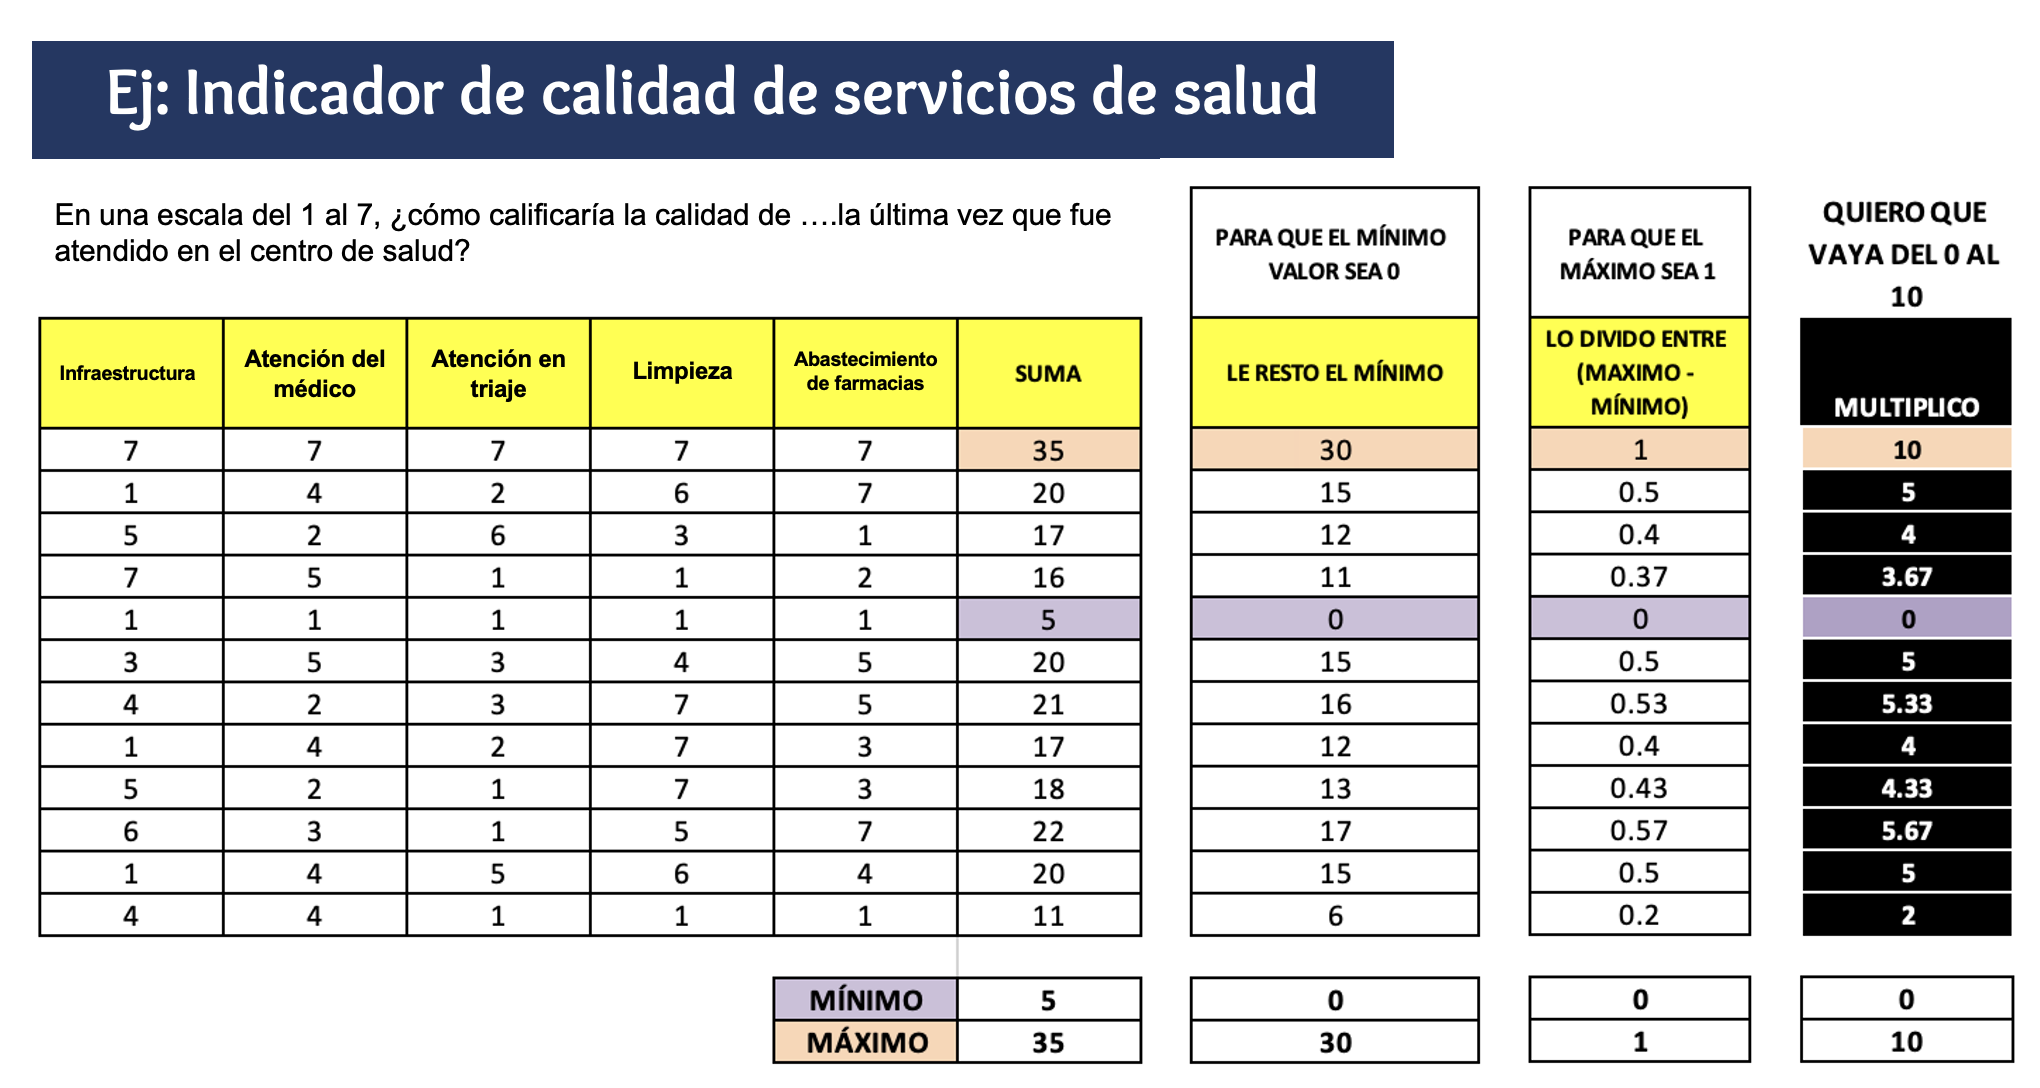
\includegraphics[width=0.6\linewidth]{pd2_ejemplo} \end{center}

Sin embargo, el paquete scales nos facilita el uso del comando
\textbf{rescale.} Al usarlo solo necesitamos señalar los límites del
indicador.

\hypertarget{pasos-para-construir-un-indicador}{%
\paragraph{Pasos para construir un
indicador:}\label{pasos-para-construir-un-indicador}}

\begin{enumerate}
\def\labelenumi{\arabic{enumi}.}
\tightlist
\item
  Verificar que las variables que construyan el indicador correspondan
  al concepto que se desea medir. \emph{Ejemplo: Si deseo mejor
  Satisfacción del Usuario, las preguntas deben ser sobre ello.}
\item
  Revisar el cuestionario e identificar el sentido de las categorías.
  \emph{Ejemplo: El valor 5 es ``Muy instafisfecho'' y 1 ``Muy
  satisfecho''}
\item
  Si las categorías de las variables están en el correcto sentido
  proceder a sumarlas, si no lo están, proceder a recodificarlas para
  luego sumar.
\item
  Una vez realizada la suma, identificar el mínimo y el máximo.
\item
  Aplicar la función \textbf{rescale} (paquete scales) con el rango
  específico.
\end{enumerate}

Construiremos un indicador aditivos de percepción de desigualdad en
calidad de vida en el Perú, que vaya del 0 al 100. Para ello usaremos a
las variables \texttt{d\_educ}, \texttt{d\_salud}, \texttt{d\_trabajo} y
\texttt{d\_justicia}.

\begin{center}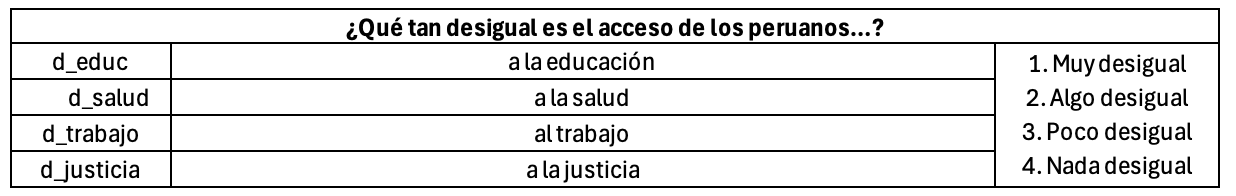
\includegraphics[width=1\linewidth]{tablitaenades2024} \end{center}

El indicador que queremos crear es de percepción de desigualdad, por
tanto mayor valor debería significar mayor desigualdad. En este caso, un
mayor valor quiere decir menos desigualdad. Debemos cambiarlo.

\begin{Shaded}
\begin{Highlighting}[]
\NormalTok{data }\OtherTok{\textless{}{-}}\NormalTok{ data }\SpecialCharTok{\%\textgreater{}\%}
  \FunctionTok{mutate}\NormalTok{(}\AttributeTok{d\_educ =} \FunctionTok{case\_when}\NormalTok{( d\_educ }\SpecialCharTok{==} \DecValTok{1} \SpecialCharTok{\textasciitilde{}} \DecValTok{4}\NormalTok{,}
\NormalTok{                            d\_educ }\SpecialCharTok{==} \DecValTok{2} \SpecialCharTok{\textasciitilde{}} \DecValTok{3}\NormalTok{,}
\NormalTok{                            d\_educ }\SpecialCharTok{==} \DecValTok{3} \SpecialCharTok{\textasciitilde{}} \DecValTok{2}\NormalTok{,}
\NormalTok{                            d\_educ }\SpecialCharTok{==} \DecValTok{4} \SpecialCharTok{\textasciitilde{}} \DecValTok{1}\NormalTok{),}
      \AttributeTok{d\_salud =} \FunctionTok{case\_when}\NormalTok{(d\_salud }\SpecialCharTok{==} \DecValTok{1} \SpecialCharTok{\textasciitilde{}} \DecValTok{4}\NormalTok{,}
\NormalTok{                          d\_salud }\SpecialCharTok{==} \DecValTok{2} \SpecialCharTok{\textasciitilde{}} \DecValTok{3}\NormalTok{,}
\NormalTok{                          d\_salud }\SpecialCharTok{==} \DecValTok{3} \SpecialCharTok{\textasciitilde{}} \DecValTok{2}\NormalTok{,}
\NormalTok{                          d\_salud }\SpecialCharTok{==} \DecValTok{4} \SpecialCharTok{\textasciitilde{}} \DecValTok{1}\NormalTok{),}
      \AttributeTok{d\_trabajo =} \FunctionTok{case\_when}\NormalTok{(d\_trabajo }\SpecialCharTok{==} \DecValTok{1} \SpecialCharTok{\textasciitilde{}} \DecValTok{4}\NormalTok{,}
\NormalTok{                            d\_trabajo }\SpecialCharTok{==} \DecValTok{2} \SpecialCharTok{\textasciitilde{}} \DecValTok{3}\NormalTok{,}
\NormalTok{                            d\_trabajo }\SpecialCharTok{==} \DecValTok{3} \SpecialCharTok{\textasciitilde{}} \DecValTok{2}\NormalTok{,}
\NormalTok{                            d\_trabajo }\SpecialCharTok{==} \DecValTok{4} \SpecialCharTok{\textasciitilde{}} \DecValTok{1}\NormalTok{),}
      \AttributeTok{d\_justicia =} \FunctionTok{case\_when}\NormalTok{(d\_justicia }\SpecialCharTok{==} \DecValTok{1} \SpecialCharTok{\textasciitilde{}} \DecValTok{4}\NormalTok{,}
\NormalTok{                             d\_justicia }\SpecialCharTok{==} \DecValTok{2} \SpecialCharTok{\textasciitilde{}} \DecValTok{3}\NormalTok{,}
\NormalTok{                             d\_justicia }\SpecialCharTok{==} \DecValTok{3} \SpecialCharTok{\textasciitilde{}} \DecValTok{2}\NormalTok{,}
\NormalTok{                             d\_justicia }\SpecialCharTok{==} \DecValTok{4} \SpecialCharTok{\textasciitilde{}} \DecValTok{1}\NormalTok{))}
\end{Highlighting}
\end{Shaded}

También podemos usar esta opción más corta. En esta le estamos pidiendo
ejecutar un cambio sa través de las cuatro variables mencionadas, y
luego mencionamos la condición. Para no repetir las cuatro variables en
cada condición podemos poner un punto (.).

\begin{Shaded}
\begin{Highlighting}[]
\NormalTok{data }\OtherTok{\textless{}{-}}\NormalTok{ data }\SpecialCharTok{\%\textgreater{}\%}
  \FunctionTok{mutate}\NormalTok{(}\FunctionTok{across}\NormalTok{(}\FunctionTok{c}\NormalTok{(d\_educ, d\_salud, d\_trabajo, d\_justicia),}
    \SpecialCharTok{\textasciitilde{}} \FunctionTok{case\_when}\NormalTok{(}
\NormalTok{        . }\SpecialCharTok{==} \DecValTok{1} \SpecialCharTok{\textasciitilde{}} \DecValTok{4}\NormalTok{,}
\NormalTok{        . }\SpecialCharTok{==} \DecValTok{2} \SpecialCharTok{\textasciitilde{}} \DecValTok{3}\NormalTok{,}
\NormalTok{        . }\SpecialCharTok{==} \DecValTok{3} \SpecialCharTok{\textasciitilde{}} \DecValTok{2}\NormalTok{,}
\NormalTok{        . }\SpecialCharTok{==} \DecValTok{4} \SpecialCharTok{\textasciitilde{}} \DecValTok{1}\NormalTok{)))}
\end{Highlighting}
\end{Shaded}

🗨️ Para poder crear el indicador, necesitamos que todas las variables a
usar sean numéricas porque las tendremos que sumar. Entonces, primero
verificamos el tipo de dato de cada variable.

\begin{Shaded}
\begin{Highlighting}[]
\FunctionTok{str}\NormalTok{(data)}
\end{Highlighting}
\end{Shaded}

\begin{verbatim}
## 'data.frame':    562 obs. of  18 variables:
##  $ edad      : num  19 40 47 20 37 27 36 37 35 19 ...
##  $ sexo      : num  1 2 2 2 2 2 2 1 1 1 ...
##  $ macrozona : num  4 3 4 4 4 4 3 4 4 4 ...
##  $ P02       : num  7 7 10 10 6 4 8 1 1 3 ...
##  $ P07       : Ord.factor w/ 4 levels "Nada"<"Poco"<..: 4 1 4 4 4 2 4 4 4 3 ...
##  $ P08       : num  1 3 1 1 1 1 2 3 1 1 ...
##  $ clase     : num  3 3 3 3 3 4 3 3 4 3 ...
##  $ P17       : num  4 2 4 3 1 3 2 1 3 3 ...
##  $ P18       : num  3 2 3 4 2 3 3 1 3 3 ...
##  $ P19       : num  4 4 4 4 4 4 3 4 3 4 ...
##  $ P20       : num  3 1 3 3 3 3 3 1 2 3 ...
##  $ P21       : num  3 2 3 3 1 1 2 1 2 3 ...
##  $ P22       : num  2 3 3 3 3 1 3 1 2 3 ...
##  $ d_educ    : num  2 3 2 1 2 1 3 1 3 2 ...
##  $ d_salud   : num  1 1 1 2 2 1 2 1 1 1 ...
##  $ d_trabajo : num  2 3 1 1 1 3 3 1 1 2 ...
##  $ d_justicia: num  2 1 2 1 2 1 2 1 1 2 ...
##  $ P37       : num  2 1 2 6 3 2 4 1 2 2 ...
\end{verbatim}

\begin{Shaded}
\begin{Highlighting}[]
\NormalTok{data}\OtherTok{=}\NormalTok{data }\SpecialCharTok{\%\textgreater{}\%}
  \FunctionTok{mutate}\NormalTok{(}\AttributeTok{suma =}\NormalTok{ d\_educ }\SpecialCharTok{+}\NormalTok{ d\_salud }\SpecialCharTok{+}\NormalTok{ d\_trabajo }\SpecialCharTok{+}\NormalTok{ d\_justicia)}
\end{Highlighting}
\end{Shaded}

Revisamos mínimo y máximo

\begin{Shaded}
\begin{Highlighting}[]
\FunctionTok{summary}\NormalTok{(data}\SpecialCharTok{$}\NormalTok{suma)}
\end{Highlighting}
\end{Shaded}

\begin{verbatim}
##    Min. 1st Qu.  Median    Mean 3rd Qu.    Max. 
##   4.000   4.000   6.000   6.306   8.000  15.000
\end{verbatim}

Creamos el indicador de 0 al 100

\begin{Shaded}
\begin{Highlighting}[]
\FunctionTok{library}\NormalTok{(scales)}
\NormalTok{data }\OtherTok{=}\NormalTok{ data }\SpecialCharTok{\%\textgreater{}\%}
  \FunctionTok{mutate}\NormalTok{(}\AttributeTok{indicador =} \FunctionTok{rescale}\NormalTok{(suma, }\AttributeTok{to =} \FunctionTok{c}\NormalTok{(}\DecValTok{0}\NormalTok{, }\DecValTok{100}\NormalTok{)))}
\end{Highlighting}
\end{Shaded}

Analicemos los descriptivos del indicador que creamos

\begin{Shaded}
\begin{Highlighting}[]
\NormalTok{data }\SpecialCharTok{\%\textgreater{}\%} 
  \FunctionTok{group\_by}\NormalTok{(clase) }\SpecialCharTok{\%\textgreater{}\%} 
  \FunctionTok{summarise}\NormalTok{(}
    \AttributeTok{Media =} \FunctionTok{mean}\NormalTok{(indicador), }
    \AttributeTok{Mediana =} \FunctionTok{median}\NormalTok{(indicador), }
    \AttributeTok{Desviacion =} \FunctionTok{sd}\NormalTok{(indicador), }
    \AttributeTok{Minimo =} \FunctionTok{min}\NormalTok{(indicador), }
    \AttributeTok{Maximo =} \FunctionTok{max}\NormalTok{(indicador),}
    \AttributeTok{Q1 =} \FunctionTok{quantile}\NormalTok{(indicador, }\FloatTok{0.25}\NormalTok{), }\CommentTok{\#Primer cuartil}
    \AttributeTok{Q3 =} \FunctionTok{quantile}\NormalTok{(indicador, }\FloatTok{0.75}\NormalTok{) }\CommentTok{\#Tercer cuartil}
\NormalTok{  )}
\end{Highlighting}
\end{Shaded}

\begin{verbatim}
## # A tibble: 4 x 8
##   clase Media Mediana Desviacion Minimo Maximo    Q1    Q3
##   <dbl> <dbl>   <dbl>      <dbl>  <dbl>  <dbl> <dbl> <dbl>
## 1     1  13.6    9.09       12.5      0   36.4  9.09  15.9
## 2     2  25.9   18.2        21.2      0   72.7  9.09  36.4
## 3     3  21.0   18.2        19.8      0   90.9  0     36.4
## 4     4  18.9    9.09       22.0      0  100    0     27.3
\end{verbatim}

\hypertarget{cuuxe1l-es-la-diferencia-de-la-percepciuxf3n-de-desigualdad-entre-clases}{%
\subsection{\texorpdfstring{4.3 ¿Cuál es la diferencia de la percepción
de desigualdad entre
\emph{clases}?}{4.3 ¿Cuál es la diferencia de la percepción de desigualdad entre clases?}}\label{cuuxe1l-es-la-diferencia-de-la-percepciuxf3n-de-desigualdad-entre-clases}}

Primero indiquemos las etiquetas de la variable. El diccionario de datos
indicaba que había 4 niveles para la variable clase. Dentro del mutate,
debemos iniciar indicando que queremos que la variable sea factor, los
niveles van del 1 al 4 y luego indicamos la etiqueta para cada nivel. La
etiqueta se otorga en el orden. En este caso el 1 será Alta, 2 será
Media alta, 3 será Media baja y 4 será Baja.

\begin{Shaded}
\begin{Highlighting}[]
\NormalTok{data }\OtherTok{=}\NormalTok{ data }\SpecialCharTok{\%\textgreater{}\%}
 \FunctionTok{mutate}\NormalTok{(}\AttributeTok{clase =} \FunctionTok{factor}\NormalTok{(clase, }\AttributeTok{levels =} \DecValTok{1}\SpecialCharTok{:}\DecValTok{4}\NormalTok{, }\AttributeTok{labels =} \FunctionTok{c}\NormalTok{(}\StringTok{"Alta"}\NormalTok{, }\StringTok{"Media alta"}\NormalTok{, }\StringTok{"Media baja"}\NormalTok{, }\StringTok{"Baja"}\NormalTok{), }\AttributeTok{ordered =} \ConstantTok{TRUE}\NormalTok{))}
\end{Highlighting}
\end{Shaded}

Para hacer la tabla resumen de los descriptivos debemos agregar la
agrupación por clase antes. Así los resultados saldrán según la clase.

\begin{Shaded}
\begin{Highlighting}[]
\NormalTok{data}\SpecialCharTok{\%\textgreater{}\%}
  \FunctionTok{group\_by}\NormalTok{(clase) }\SpecialCharTok{\%\textgreater{}\%}
  \FunctionTok{summarise}\NormalTok{(}
    \AttributeTok{Media =} \FunctionTok{mean}\NormalTok{(indicador), }
    \AttributeTok{Mediana =} \FunctionTok{median}\NormalTok{(indicador), }
    \AttributeTok{Desviacion =} \FunctionTok{sd}\NormalTok{(indicador), }
    \AttributeTok{Minimo =} \FunctionTok{min}\NormalTok{(indicador), }
    \AttributeTok{Maximo =} \FunctionTok{max}\NormalTok{(indicador),}
    \AttributeTok{Q1 =} \FunctionTok{quantile}\NormalTok{(indicador, }\FloatTok{0.25}\NormalTok{), }\CommentTok{\#Primer cuartil}
    \AttributeTok{Q3 =} \FunctionTok{quantile}\NormalTok{(indicador, }\FloatTok{0.75}\NormalTok{) }\CommentTok{\#Tercer cuartil}
\NormalTok{  )}
\end{Highlighting}
\end{Shaded}

\begin{verbatim}
## # A tibble: 4 x 8
##   clase      Media Mediana Desviacion Minimo Maximo    Q1    Q3
##   <ord>      <dbl>   <dbl>      <dbl>  <dbl>  <dbl> <dbl> <dbl>
## 1 Alta        13.6    9.09       12.5      0   36.4  9.09  15.9
## 2 Media alta  25.9   18.2        21.2      0   72.7  9.09  36.4
## 3 Media baja  21.0   18.2        19.8      0   90.9  0     36.4
## 4 Baja        18.9    9.09       22.0      0  100    0     27.3
\end{verbatim}

\begin{Shaded}
\begin{Highlighting}[]
\FunctionTok{ggplot}\NormalTok{(data, }\FunctionTok{aes}\NormalTok{(}\AttributeTok{x=}\NormalTok{clase, }\AttributeTok{y=}\NormalTok{indicador, }\AttributeTok{color=}\NormalTok{clase)) }\SpecialCharTok{+} 
  \FunctionTok{geom\_boxplot}\NormalTok{() }\SpecialCharTok{+} 
  \FunctionTok{geom\_jitter}\NormalTok{(}\AttributeTok{shape=}\DecValTok{16}\NormalTok{, }\AttributeTok{position=}\FunctionTok{position\_jitter}\NormalTok{(}\FloatTok{0.2}\NormalTok{),}\AttributeTok{alpha=}\FloatTok{0.6}\NormalTok{) }\SpecialCharTok{+}\CommentTok{\#para agregar los casos como puntos}
  \FunctionTok{theme\_classic}\NormalTok{()}
\end{Highlighting}
\end{Shaded}

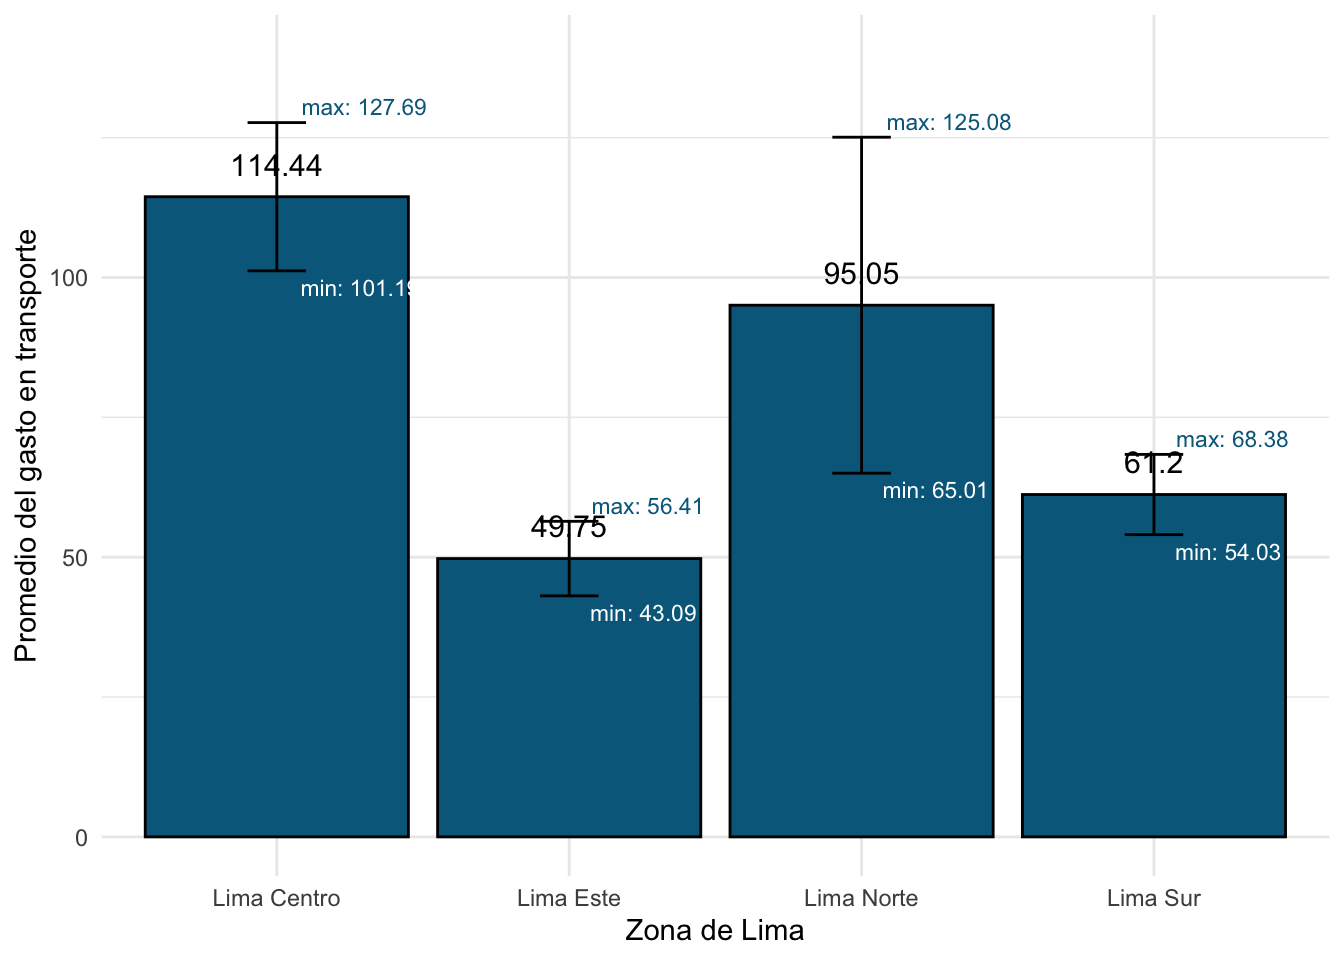
\includegraphics{pd2_files/figure-latex/unnamed-chunk-30-1.pdf}

➡️ Análisis: En el segundo gráfico la dispersión de los datos es muy
similar en el grupo de clase social Media baja y Baja. Por otro lado, en
el grupo de la clase Alta, se aprecia que la dispersión es mucho mayor
(la caja es mucho más grande). Los \emph{outliers} se muestran como
puntos individuales más allá del bigote de la caja, los puntos más
alejados se encuentran en el grupo de clase Baja.

\hypertarget{ejercicios}{%
\section{\texorpdfstring{\textbf{5.
Ejercicios}}{5. Ejercicios}}\label{ejercicios}}

\begin{enumerate}
\def\labelenumi{\arabic{enumi}.}
\item
  Analiza los descriptivos de la variable P08. Recuerda determinar
  primero qué tipo de variable es. Realiza el gráfico correspondiente e
  interpreta.
\item
  Analiza los descriptivos de la variable P37. Recuerda determinar
  primero qué tipo de variable es. Realiza el gráfico correspondiente e
  interpreta.
\item
  Crea el indicador de percepción de gravedad de desigualdad
  socioeconómica en el Perú. Para ello usa las variables P17, P18, P19,
  P20, P21 y P22. El indicador debe ir del del 0 al 10, en donde 0 sea
  nada grave y 10 sea muy grave. No olvides revisar el sentido de cada
  pregunta.
\item
  Con el indicador creado previamente, realiza el gráfico pertinente e
  interpreta.
\end{enumerate}

\end{document}
